\section{Archimate 2.0}

Según  \cite{archimate2}, archimate es un lenguaje estandar utilizado por los arquitectos de software para modelar las necesidades de cada \textit{stakeholder}, dividiendo el contexto en el que se desenvuelve el software a desarrollar en tres capas: capa de negocio, capa de aplicación y capa de infraestructura.

\subsection{Capas de archimate}

A continuación serán descritas las tres capas definidas en el estandar archimate.

\subsubsection{Capa de negocio}

Esta capa envuelve todos los conceptos relacionados con la organización sobre la cual se aplicará el software a desarrollar, esto es, los roles, los servicios ofrecidos, los procesos, los productos y demás conceptos aplicados sobre su estructura y dinámica.

Artefactos***********

A continuación se hará un sumario de los artefactos utilizados en el presente proyecto para modelar la arquitectura a seguir:

\begin{table}
  \caption{Artefactos de la capa de negocio}
  \label{tab:artefactos_capa_negocio}

  \begin{center}
  
  \textbf{Fuente:} \cite{archimate2}
  
  \resizebox{15cm}{!}{
  \begin{tabular}{|L{1cm}L{3cm}c|}
    \hline
    \multicolumn{1}{c}{Artefacto} & \multicolumn{1}{c}{Descripción} & \multicolumn{1}{c}{Notación} \\ 
    \hline
    \multicolumn{1}{c}{\textit{Actor de negocio (Business actor)}} & 
    \multicolumn{1}{c}{Ente (persona) organizacional quien cumple tareas en la organización} &  
    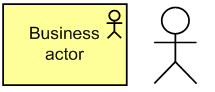
\includegraphics[width=7cm]{./imagenes/Archimate/businessactor.png}\\
    %\begin{figure}[!htb]
  	%	\begin{center}
    %		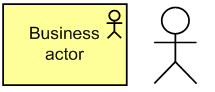
\includegraphics[width=11cm]{./imagenes/Archimate/businessactor.png}
    %		\label{fig:businessactor}
    %		\textbf{Fuente:}  \cite{archimate2}
  	%	\end{center}
	%\end{figure}  
	\hline
	\multicolumn{1}{c}{\textit{Colaboración de negocio (Business collaboration)}} & 
    \multicolumn{1}{c}{Rol que surge de la combinación de dos o más roles} &  
    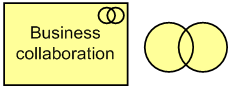
\includegraphics[width=7cm]{./imagenes/Archimate/businesscollaboration.png}\\
    \hline
  \end{tabular}
  }
    \end{center}
\end{table}